\section{Related Work}
\label{related}

\noindent \textbf{KV cache reuse.}
%Some works~\cite{alluneed-nips17, scaling-mlsys23, vllm-sosp23, flexgen-icml23} focus on reusing previously stored KV caches across different iterations within a request to reduce computation, and optimized memory allocation to support larger KV cache at runtime. These efforts target reducing decoding phase and are orthogonal to \pname{} which targets  prefill phase. Combining them with \pname{} can further accelerate the whole inference process.
%Recent studies~\cite{attentionstore-atc24, chunkattention-arxiv24, hydragen-arxiv24, ragcache-arxiv24, sglang-arxiv23, cachegen-sigcomm24} reuse shared prefix KV caches across different requests to reduce prefill latency (i.e., TTFT). However, these works load the entire prefix KVs, leading to high I/O latency when the KVs are stored on disk. In contrast, \pname{} prefetches only important prefix KVs, reducing I/O latency. 
%Other efforts~\cite{promptcache-mlsys24, cacheblend-arxiv24} explore finer-grained reuse of prefix KVs at the text segment level, which is orthogonal to \pname{} and can be combined to enable more KV reuse.
\fvc{
Some works~\cite{alluneed-nips17, scaling-mlsys23, vllm-sosp23, flexgen-icml23} accelerate the decoding phase by reusing KVs across iterations within a request. These are orthogonal to \pname{}, which targets the prefill phase.
Recent studies~\cite{attentionstore-atc24, chunkattention-arxiv24, hydragen-arxiv24, ragcache-arxiv24, sglang-arxiv23, cachegen-sigcomm24} reuse shared prefix KVs across requests to reduce prefill latency (i.e., TTFT), but load entire prefix KVs, causing high I/O latency when KVs are on disk. In contrast, \pname{} prefetches only important prefix KVs, reducing I/O latency. 
Other efforts~\cite{promptcache-mlsys24, cacheblend-arxiv24} explore finer-grained reuse of prefix KVs at the text segment level, which is orthogonal to \pname{} and can be combined to enable more KV reuse.
}


\begin{figure}
	\centering
	\begin{minipage}{1.6in}
		% \centering
		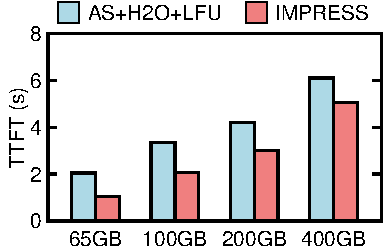
\includegraphics[width=1.6in,height=1in]{sens_datasetsize.pdf}
		\vspace{-0.1in}
		\caption{
			\fv{Results on various dataset sizes.}
		}
		\label{fig:sens_datasetsize}
	\end{minipage}
	\hspace{0.04in}
	\begin{minipage}{1.6in}
		\centering
		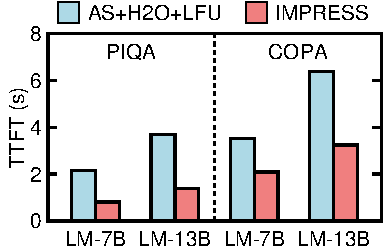
\includegraphics[width=1.6in, height=1in]{sens_llama.pdf}
		\vspace{-0.1in}
		\caption{
			\fv{Results on Llama (LM) models.}
		}
		\label{fig:sens_modeltype}
	\end{minipage} 
	\vspace{-0.15in}
\end{figure}

\noindent \textbf{KV pruning and quantization.}
%Recent studies~\cite{scissorhands-nips23, flexgen-icml23, h2o-nips23, infinigen-osdi24} demonstrate that LLM inference can achieve comparable output quality using only a subset of important KVs, proposing various algorithms to better predict and identify these KVs. However, they require the full keys during the prefill phase, which makes them suboptimal when directly combined with prefix KV storage systems due to the high I/O load. 
%In contrast, \pname{} leverages the similarity of important token indices across heads, allowing the identification of important KVs with minimal I/O, reducing TTFT while maintaining high accuracy.
%Other works~\cite{flexgen-icml23, cachegen-sigcomm24, kivi-arxiv24, kvquant-arxiv24, wkvquant-arxiv24} focus on quantizing KVs to reduce the bit count needed for each key and value element. These quantization techniques can be applied alongside \pname{} to further decrease data load.
\fvc{
Recent studies~\cite{scissorhands-nips23, flexgen-icml23, h2o-nips23, infinigen-osdi24} show LLM inference can achieve similar output quality using only a subset of KVs, proposing various methods to identify these KVs. 
However, they require full keys during the prefill phase, leading to high I/O latency when combined with prefix KV storage systems. 
\pname{} leverages the similarity of important token indices across heads to identify important KVs with minimal I/O, reducing TTFT while maintaining high accuracy. 
}
%Others~\cite{flexgen-icml23, cachegen-sigcomm24, kivi-arxiv24, kvquant-arxiv24, wkvquant-arxiv24} focus on quantizing KVs to reduce the bit count for each key and value element. These quantization techniques can be applied alongside \pname{} to further decrease data load.
\fvc{
Others~\cite{flexgen-icml23, cachegen-sigcomm24, kivi-arxiv24, kvquant-arxiv24, wkvquant-arxiv24} focus on KV quantization to reduce bit counts per key and value element. They can complement \pname{} to further decrease data load.
}


\noindent \textbf{Other efficient LLM serving systems.}
Some works optimize other aspects of inference systems, such as request scheduling~\cite{orca-osdi22, taming-osdi24}, model parallelism strategies~\cite{alpaserve-osdi23, loongserve-arxiv24}, prefill-decoding decoupling~\cite{distserve-osdi24, splitwise-isca24, pdserve-arxiv24, tetriinf-arxiv24, dv-arxiv24}, and distributed KV cache~\cite{infinite-arxiv24, mooncake-arxiv24}. These optimizations are also orthogonal to \pname{} and can complement its improvements.
